\documentclass[border=8pt]{standalone}
\usepackage{tikz}
\usepackage{xcolor}
\usetikzlibrary{positioning,arrows.meta,calc}

\definecolor{zombFill}{HTML}{FDDBC7}
\definecolor{zombEdge}{HTML}{B2182B}
\definecolor{transFill}{HTML}{D1E5F0}
\definecolor{transEdge}{HTML}{2166AC}
\definecolor{neutFill}{HTML}{F0F0F0}
\definecolor{neutEdge}{HTML}{6E6E6E}

\begin{document}
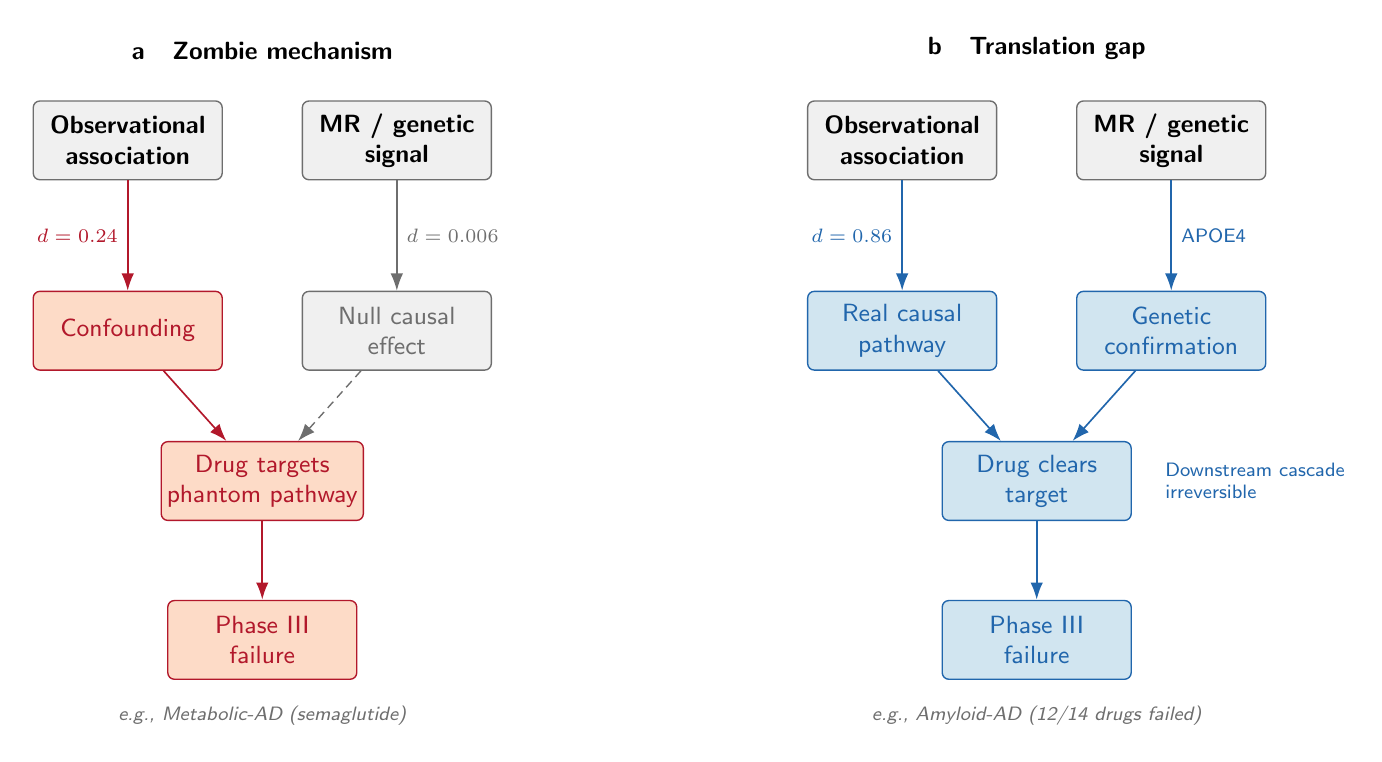
\begin{tikzpicture}[
    >={Latex[length=2.2mm,width=1.6mm]},
    font=\sffamily\small,
    node distance=11mm and 6mm,
    base/.style={rounded corners=2.4pt, draw, line width=0.5pt,
      minimum width=24mm, minimum height=10mm, align=center, inner sep=2pt},
    zombie/.style={base, fill=zombFill, draw=zombEdge, text=zombEdge},
    trans/.style={base, fill=transFill, draw=transEdge, text=transEdge},
    neut/.style={base, fill=neutFill, draw=neutEdge, text=neutEdge},
    bold/.style={base, fill=neutFill, draw=neutEdge, text=black, font=\sffamily\small\bfseries},
    zarr/.style={->, draw=zombEdge, line width=0.6pt},
    tarr/.style={->, draw=transEdge, line width=0.6pt},
    garr/.style={->, draw=neutEdge, line width=0.5pt},
    panel/.style={font=\sffamily\small\bfseries, text=black},
  ]

% ===== PANEL a — Zombie mechanism =====
\node[bold] (aObs) {Observational\\association};
\node[bold, right=10mm of aObs] (aMR) {MR / genetic\\signal};
\node[zombie, below=14mm of aObs] (aConf) {Confounding};
\node[neut, below=14mm of aMR] (aNull) {Null causal\\effect};

\coordinate (aMid) at ($(aConf)!0.5!(aNull)$);
\node[zombie, below=14mm of aMid] (aDrug) {Drug targets\\phantom pathway};
\node[zombie, below=10mm of aDrug] (aFail) {Phase III\\failure};

% Arrows
\draw[zarr] (aObs) -- node[left, font=\sffamily\scriptsize, text=zombEdge] {$d = 0.24$} (aConf);
\draw[garr] (aMR) -- node[right, font=\sffamily\scriptsize, text=neutEdge] {$d = 0.006$} (aNull);
\draw[zarr] (aConf) -- (aDrug);
\draw[garr, densely dashed] (aNull) -- (aDrug);
\draw[zarr, line width=0.8pt] (aDrug) -- (aFail);

% Panel label
\node[panel, above=4mm of $(aObs.north)!0.5!(aMR.north)$] {\textbf{a}\quad Zombie mechanism};
\node[below=2mm of aFail, font=\sffamily\scriptsize\itshape, text=neutEdge] {e.g., Metabolic-AD (semaglutide)};

% ===== PANEL b — Translation gap =====
\node[bold, right=40mm of aMR] (bObs) {Observational\\association};
\node[bold, right=10mm of bObs] (bMR) {MR / genetic\\signal};
\node[trans, below=14mm of bObs] (bReal) {Real causal\\pathway};
\node[trans, below=14mm of bMR] (bGen) {Genetic\\confirmation};

\coordinate (bMid) at ($(bReal)!0.5!(bGen)$);
\node[trans, below=14mm of bMid] (bDrug) {Drug clears\\target};
\node[trans, below=10mm of bDrug] (bFail) {Phase III\\failure};

% Arrows
\draw[tarr] (bObs) -- node[left, font=\sffamily\scriptsize, text=transEdge] {$d = 0.86$} (bReal);
\draw[tarr] (bMR) -- node[right, font=\sffamily\scriptsize, text=transEdge] {APOE4} (bGen);
\draw[tarr] (bReal) -- (bDrug);
\draw[tarr] (bGen) -- (bDrug);
\draw[tarr, line width=0.8pt] (bDrug) -- (bFail);

% Translation gap annotation
\node[right=3mm of bDrug, font=\sffamily\scriptsize, text=transEdge, align=left]
  {Downstream cascade\\irreversible};

% Panel label
\node[panel, above=4mm of $(bObs.north)!0.5!(bMR.north)$] {\textbf{b}\quad Translation gap};
\node[below=2mm of bFail, font=\sffamily\scriptsize\itshape, text=neutEdge] {e.g., Amyloid-AD (12/14 drugs failed)};

\end{tikzpicture}
\end{document}
